%slide di introduzione ai fondamenti di Document Type Definition
%frame 01
%\begin{frame}
%    \frametitle{Elementi per la definizione degli schemi xml}
%    \framesubtitle{Principi Document Type Definition}
%    \addtocounter{nframe}{1}
%
%    \begin{block}{Esempio DTD}
%        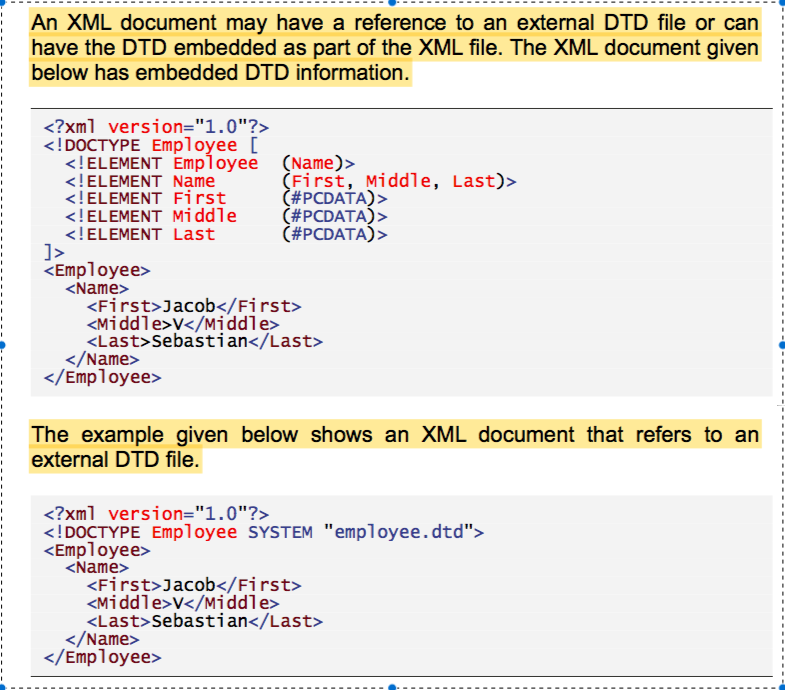
\includegraphics[width=.8\textwidth]{imgs/dtd.png}
%    \end{block}
% \end{frame}

\begin{frame}
    \frametitle{Elementi per la definizione degli schemi xml}
    \framesubtitle{Principi Document Type Definition}
    \addtocounter{nframe}{1}

    \begin{block}{Document Type Definition (DTD)}
        Una document type definition (DTD) descrive le regole relative alla struttura di un documento XML.
    \end{block}

    \begin{block}{Document Type Definition (DTD)}
        Una DTD dichiara gli elementi, gli attributi, le entità e le notazioni ammesse in un documento XML.
    \end{block}

\end{frame}


\begin{frame}
    \frametitle{Elementi per la definizione degli schemi xml}
    \framesubtitle{Principi Document Type Definition}
    \addtocounter{nframe}{1}

    \begin{block}{well-formed document != valid document}
         Se un documento XML manca di riferirsi ad una DTD oppure non rispetta le regole di una DTD, esso può essere tutt'al più ben formato, ma sicuramente non può essere valido.
    \end{block}
\end{frame}

\begin{frame}
    \frametitle{Elementi per la definizione degli schemi xml}
    \framesubtitle{Principi Document Type Definition}
    \addtocounter{nframe}{1}

    \begin{block}{Document Type Definition (DTD)}
        La validazione dei documenti XML è alla base della condivisione e scambio dati in quanto è possibile confidare sulla natura dei dati trasmessi.
    \end{block}
   \textit{Attenzione: non possiamo validare la correttezza della semantica dei dati!}
\end{frame}

\begin{frame}
    \frametitle{Elementi per la definizione degli schemi xml}
    \framesubtitle{Principi Document Type Definition}
    \addtocounter{nframe}{1}

    \begin{block}{Document Type Definition (DTD)}
         L'associazione tra documento XML e DTD viene realizzata tramite una dichiarazione inclusa nel prologo all'inizio del documento.
    \end{block}

    \begin{block}{Root element and content}
        La DTD dichiara l'elemento radice del vocabolario e il suo \textit{content model} (children elements).
    \end{block}
   
\end{frame}

\begin{frame}
    \frametitle{Elementi per la definizione degli schemi xml}
    \framesubtitle{Principi Document Type Definition}
    \addtocounter{nframe}{1}

    \begin{block}{Element Declaration (con figli)}
        \begin{center}\texttt{<!ELEMENT element-name (child-element1, child-element-2 ...)>}\end{center}
    \end{block}

    \begin{block}{Element Declaration (solo testo)}
    \begin{center}\texttt{<!ELEMENT element-name (\#PCDATA)>}\end{center}
    \end{block}
    \textit{Il Parsed Character Content designa contenuto testuale piano senza figli}
\end{frame}

\begin{frame}
    \frametitle{Elementi per la definizione degli schemi xml}
    \framesubtitle{Principi Document Type Definition}
    \addtocounter{nframe}{1}

    \begin{block}{Child Element Declaration}
        La dichiarazione di un elemento figlio, è analoga in tutto e per tutto alla dichiarazione dell'elemento radice. Cioè utilizzando l'etichetta \texttt{<!ELEMENT >}
    \end{block}

    \begin{block}{Element Declaration (root)}
     \textbf{La dichiarazione dell'elemento radice deve sempre essere la prima}
    \end{block}
\end{frame}

\begin{frame}
    \frametitle{Elementi per la definizione degli schemi xml}
    \framesubtitle{Principi Document Type Definition}
    \addtocounter{nframe}{1}

    \begin{block}{Modificatori}
        Nella dichiarazione di un elemento possono essere inclusi opzionalmente dei modificatori, per stabilire il numero di occorrenze degli elementi figli.
    \end{block}

    \begin{block}{Modificatori}
     + Una o più occorrenze\\ 
     ? Zero o una occorrenza\\
     * Zero o più occorrenze
    \end{block}
\end{frame}

\begin{frame}
    \frametitle{Elementi per la definizione degli schemi xml}
    \framesubtitle{Principi Document Type Definition}
    \addtocounter{nframe}{1}

    \begin{block}{Modificatori}
        \begin{center} \texttt{<!ELEMENT element-name (B, C)+ >} \end{center}
        \begin{center} \texttt{<!ELEMENT element-name (B+, C) >} \end{center}
        \begin{center} \texttt{<!ELEMENT element-name (B, C+) >} \end{center}
        \begin{center} \texttt{<!ELEMENT element-name (B+, C+) >} \end{center}
    \end{block}

     \textit{Se un elemento figlio deve presentarsi solo una volta, allora non c'è bisogno di modificatori}.
     \\\textit{Attenzione l'ordine dei figli nella dichiarazione è significativa}
    
\end{frame}

\begin{frame}
    \frametitle{Elementi per la definizione degli schemi xml}
    \framesubtitle{Principi Document Type Definition}
    \addtocounter{nframe}{1}

    \begin{block}{Esercizio}
        \textit{Definire i seguenti elementi:}
        \begin{itemize}
            \item elemento root: \textbf{TEI}
            \item elementi figli:
            \begin{itemize}
                \item header (obbligatorio una occorrenza)
                \item facsimile (opzionale una occorrenza)
                \item text (obbligatorio almeno una occorrenza)
            \end{itemize}
        \end{itemize}
        \textit{Gli elementi header, facsimile e text hanno tutti un content model testuale}
    \end{block}
\end{frame}


\begin{frame}
    \frametitle{Elementi per la definizione degli schemi xml}
    \framesubtitle{Principi Document Type Definition}
    \addtocounter{nframe}{1}

    \begin{block}{choice declaration}
    \begin{center} \texttt{<!ELEMENT element-name (child-a | child-b) >} \end{center}
    \end{block}

    \begin{block}{Dichiarazione di Choice}
        La sintassi della DTD consente di dichiarare una scelta (\textit{choice}) tra due o più elementi come content model di un elemento. 
        \\ \textit{Il choice indica una scelta tra una lista di possibilità}
    \end{block}

\end{frame}

\begin{frame}
    \frametitle{Elementi per la definizione degli schemi xml}
    \framesubtitle{Principi Document Type Definition}
    \addtocounter{nframe}{1}

    \begin{block}{Attributi degli elementi XML}
    \begin{center} Un attributo è dichiarato sfruttando l'elemento \texttt{<!ATTLIST >} \end{center}
    \end{block}

    \begin{block}{Cos'è un attributo di un elemento XML}
        Un attributo è una proprietà, una caratteristica di un elemento e descrive il contenuto dell'elemento stesso.
    \end{block}

\end{frame}

\begin{frame}
    \frametitle{Elementi per la definizione degli schemi xml}
    \framesubtitle{Principi Document Type Definition}
    \addtocounter{nframe}{1}

    \begin{block}{Attributi: sintassi}
    \begin{center} \texttt{<!ATTLIST Element-name Attr-name Attr-type Attr-state? default-value?>} \end{center}
    \end{block}

\end{frame}


\begin{frame}
    \frametitle{Elementi per la definizione degli schemi xml}
    \framesubtitle{Principi Document Type Definition}
    \addtocounter{nframe}{1}

    \begin{block}{Attributi: sintassi}
        \begin{itemize}
            \item ``Element-name'' è il nome dell'elemento a cui l'atteibuto si riferisce
            \item ``Attr-name'' è il nome dell'attributo dichiarato
            \item ``Attr-type'' è il tipo di dato atteso dell'attributo
            \item ``Attr-state'' indica uno tra i tre stati possibili di un attributo 
            \item ``default-value'' indica il valore di default per quell'attributo, se non fornito.
        \end{itemize}
    \end{block}

\end{frame}



\begin{frame}
    \frametitle{Elementi per la definizione degli schemi xml}
    \framesubtitle{TABELLA dei tipi}
    \addtocounter{nframe}{1}

    \begin{center}
        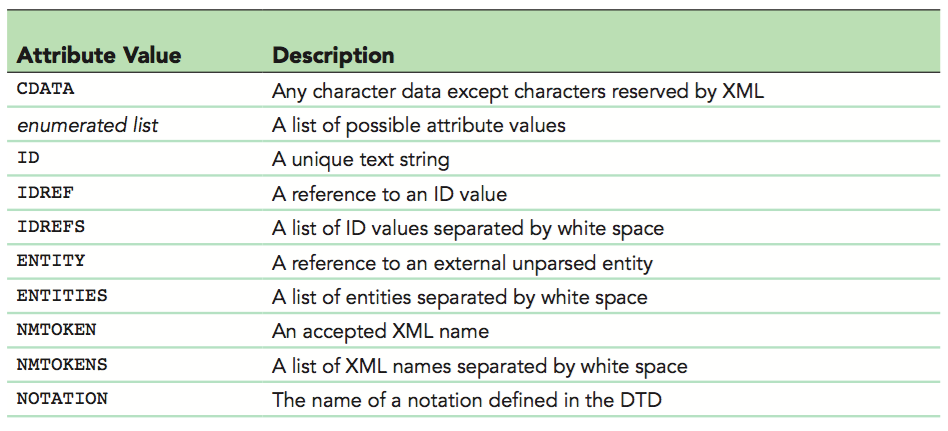
\includegraphics[width=.95\textwidth]{imgs/xml-TipiAttributoXML.png}
    \end{center}
\end{frame}


\begin{frame}
    \frametitle{Elementi per la definizione degli schemi xml}
    \framesubtitle{}
    \addtocounter{nframe}{1}

    \begin{block}{Stato di attributi}
        Lo stato di un attributo può essere uno tra:
        \begin{itemize}
            \item \#IMPLIED (attributo opzionale)
            \item \#REQUIRED (attributo obbligatorio)
            \item \#FIXED (valore fisso dell'attributo)
        \end{itemize}
    \end{block}
    \textit{Il valore di un attributo fisso viene fornito come valore di default}
\end{frame}

% slide con choice per gli attributi Enumerated Type

\begin{frame}
    \frametitle{Elementi per la definizione degli schemi xml}
    \framesubtitle{}
    \addtocounter{nframe}{1}

    \begin{block}{Choice attributi}
     \texttt{<!ATTLIST element attribute (value1 | value2 | value3 | ...) default >}
    \\\texttt{<!ATTLIST name title (Mr. | Mrs. | Ms.) \#IMPLIED ``Mr.''>}
    \end{block}
    \textit{Attenzione non è possibile avere un valore di default se un attributo è marcato \#REQUIRED}
\end{frame}

% slide con esempio ID IDREF e IDREFS
\begin{frame}
    \frametitle{Elementi per la definizione degli schemi xml}
    \framesubtitle{}
    \addtocounter{nframe}{1}

    \begin{block}{Attributi ID IDREF IDREFS}
     \texttt{<!ATTLIST element attribute ID  >}
    \\\texttt{<!ATTLIST order orderID ID \#REQUIRED>}
    \\\texttt{<!ATTLIST customer orders IDREFS>}
    \\\texttt{<!ATTLIST package orderRef IDREF>}
    \end{block}
\end{frame}

\begin{frame}
    \frametitle{Elementi per la definizione degli schemi xml}
    \framesubtitle{}
    \addtocounter{nframe}{1}

    \begin{block}{Mixed content - DTD}
    \begin{center}\texttt{<!ELEMENT element-name (\#PCDATA|child-element)* >}\end{center}
    \end{block}

    \begin{block}{Mixed content XML}
    \begin{center}\texttt{<p>Ieri pomeriggio sono andato a <placeName>Pisa</placeName>, per un giro</p>}\end{center}
    \end{block}

\end{frame}


\begin{frame}
    \frametitle{Elementi per la definizione degli schemi xml}
    \framesubtitle{}
    \addtocounter{nframe}{1}

    \begin{block}{Esercizio}
        root: TEI
         \\Figli: 
         \\- header(obbligatorio una volta sola) 
         \\- facsimile(opzionale una volta sola) 
         \\- testo(obbligatorio una o più volte)
         \\ * testo è un mixed content con possibile elemento \texttt{<seg>} 
         \\Attributi: 
         \\- header: type:(fixed, CDATA ``intestazione''); lang(opzionale, NMTOKEN)
         \\- facsimile: source:(obbligatorio); ref(optionale, IDREFS)
         \\- testo: id(obbligatorio, ID) type(opzionale contenuto testuale)
    \end{block}
\end{frame}

\begin{frame}
    \frametitle{Elementi per la definizione degli schemi xml}
    \framesubtitle{Principi Document Type Definition}
    \addtocounter{nframe}{1}

    \begin{block}{Empty elements}
        Un elemento XML può essere vuoto (empty). La dichiarazione di un elemento vuoto si realizza con la parola chiave \textbf{EMPTY}.
    \end{block}

    \begin{block}{Empy content}
    \begin{center}\texttt{<!ELEMENT element-name EMPTY>}\end{center}
    \end{block}

    \begin{block}{Empy content}
        \begin{center}
            \texttt{<!ELEMENT lb EMPTY>}
            \\\texttt{<lb />}
        \end{center}
    \end{block}

\end{frame}


\begin{frame}
    \frametitle{Elementi per la definizione degli schemi xml}
    \framesubtitle{Principi Document Type Definition}
    \addtocounter{nframe}{1}

    \begin{block}{Any elements}
        E' possibile dichiarare anche elementi che hanno qualsiasi tipo di content model.
        \\ A tal proposito viene impiegata la parola chiave  ``ANY''.
    \end{block}

    \begin{block}{Any content}
    \begin{center}\texttt{<!ELEMENT element-name ANY >}\end{center}
    \end{block}
    
\end{frame}

\begin{frame}
    \frametitle{Elementi per la definizione degli schemi xml}
    \framesubtitle{Principi Document Type Definition}
    \addtocounter{nframe}{1}

    \begin{block}{Dichiarare il tipo del documento XML}
        La dichiarazione della DTD viene inserita attraverso una URL nel prologo del documento XML, tra la dichiarazione del documento XML e l'elemento radice.
    \end{block}

    \begin{block}{Dichiarare il tipo del documento XML}
        Grazie al sistema di dichiarazione della DTD è possibile massimizzare il riuso e collegare lo schema a tutti i documenti che si vuole validare.
    \end{block}

\end{frame}

\begin{frame}
    \frametitle{Elementi per la definizione degli schemi xml}
    \framesubtitle{Principi Document Type Definition}
    \addtocounter{nframe}{1}

    \begin{block}{DOCTYPE}
    \begin{center}\texttt{<!DOCTYPE root-element SYSTEM ``External DTD’s URL'' [Internal DTD ]>}\end{center}
    \begin{center}\texttt{<!DOCTYPE root-element [Internal DTD] >}\end{center}
    \begin{center}\texttt{<!DOCTYPE root-element SYSTEM ``Ext-DTD URL'' >}\end{center}
        
    \end{block}

\end{frame}

% includere DTD pubbliche

\begin{frame}
    \frametitle{Elementi per la definizione degli schemi xml}
    \framesubtitle{Principi Document Type Definition}
    \addtocounter{nframe}{1}

    \begin{block}{DOCTYPE PUBLIC}
    \begin{center}\texttt{<!DOCTYPE root PUBLIC “id” “uri”>}\end{center}
    \begin{center}\texttt{standard//owner//description//language}\end{center}
    \begin{center}\texttt{-//W3C//DTD XHTML 1.0 Strict//EN}\end{center}
        
    \end{block}

\end{frame}

\begin{frame}
    \frametitle{Elementi per la definizione degli schemi xml}
    \framesubtitle{Principi Document Type Definition}
    \addtocounter{nframe}{1}

    \begin{block}{Esercizi}
    \begin{itemize}
        \item includere all'interno di un documento XML la dichiarazione del tipo, definire internamente gli elementi e gli attributi e validare.
        \item inserire nel prologo di un documento XML la dichiarazione del tipo di documento e validare.
    \end{itemize}
    \end{block}

    \textit{Creare un file esterno con estensione .dtd prima di includerlo nel prologo XML.}

\end{frame}


\begin{frame}
    \frametitle{Elementi per la definizione degli schemi xml}
    \framesubtitle{Principi Document Type Definition}
    \addtocounter{nframe}{1}

    \begin{block}{Entity}
        Per includere dati da diverse fonti, DTD prevede l'uso di entità. Due tipologie di entità sono state definite: general entities e parameter entities.
    \end{block}

    \begin{block}{Entity: generiche e parametriche}
    \begin{itemize}
        \item le general entities vengono espanse nel documento XML
        \item le parameter entities vengono espanse nel documento DTD
    \end{itemize}
    \end{block}
    
\end{frame}

\begin{frame}
    \frametitle{Elementi per la definizione degli schemi xml}
    \framesubtitle{Principi Document Type Definition}
    \addtocounter{nframe}{1}

    \begin{block}{Entity}
    \begin{itemize}
        \item  Le general entities si possono classificare in interne ed esterne, a loro volta possono essere parsed oppure unparsed.
        \item Le parameter entities si possono classificare in interne ed esterne; che  possono essere solo parsed.
    \end{itemize}
    \end{block}
    
\end{frame}

\begin{frame}
    \frametitle{Elementi per la definizione degli schemi xml}
    \framesubtitle{Principi Document Type Definition}
    \addtocounter{nframe}{1}

    \begin{block}{Entity}
     Le entità generiche interne aiutano ad includere nel documento XML quei caratteri speciali che altrimenti causerebbero errori al passaggio del parser.
    \end{block}

    \begin{block}{Internal General Entity: Sintassi}
    \begin{center}\texttt{<!ENTITY entity-name ``replacement-string'' or ``hexadecimal-code'' >}\end{center}
    \end{block}

\end{frame}


\begin{frame}
    \frametitle{Elementi per la definizione degli schemi xml}
    \framesubtitle{Principi Document Type Definition}
    \addtocounter{nframe}{1}

    \begin{block}{Internal General Entity: Sintassi}
        Per usare le entità all'interno del documento XML basta prefissare al nome dell'entità una ``e commerciale'' \textbf{(\&)} e aggiungere alla fine come suffisso un ``punto e virgola'' \textbf{(;)}:  \texttt{\&entity-name;}.
        \\ \textit{Una entità può contenere un frammento XML ben formato}
    \end{block}

    \begin{block}{Internal General Entity: Sintassi}
    \begin{center}\texttt{<!ENTITY firma ``<i>Angelo Mario Del Grosso</i>''>}\end{center}
    \begin{center}\texttt{<p><salutation>\&firma;<salutation></p>}\end{center}
    \end{block}

\end{frame}

\begin{frame}
    \frametitle{Elementi per la definizione degli schemi xml}
    \framesubtitle{Principi Document Type Definition}
    \addtocounter{nframe}{1}

    \begin{block}{Internal General Entity: Esempio con UNICODE}
        Spesso le entità vengono utlizzate per dare un nome ai riferimenti a carattere.
    \end{block}

    \begin{block}{Internal General Entity: Sintassi}
    \begin{center}\texttt{<!ENTITY amaiuscola ``\&\#65;''>}\end{center}
    \begin{center}\texttt{<!ENTITY amaiuscola ``\&\#x0041;''>}\end{center}
    \begin{center}\texttt{<p><salutation>\&amaiuscola;ddio<salutation></p>}\end{center}
    \end{block}

\end{frame}

\begin{frame}
    \frametitle{Elementi per la definizione degli schemi xml}
    \framesubtitle{Principi Document Type Definition}
    \addtocounter{nframe}{1}

    \begin{block}{External General Entity}
        Un documento XML può essere composto da altri pezzi di XML distribuiti in diversi luoghi. 
        \\Grazie alle entità generiche esterne è stata implementata questa caratteristica.
    \end{block}

    \begin{block}{External General Entity: Sintassi}
    \begin{center}\texttt{<!ENTITY entity-name SYSTEM ``URL'' >}\end{center}
    \begin{center}\texttt{<!ENTITY salutation SYSTEM ``salut.xml.ent'' >}\end{center}
    \end{block}
    \textit{L'URL punta al luogo dove risiede la external entity}
\end{frame}

\begin{frame}
    \frametitle{Elementi per la definizione degli schemi xml}
    \framesubtitle{Principi Document Type Definition}
    \addtocounter{nframe}{1}

    \begin{block}{External General Entity}
        Le entità esterne non possono contenere una DTD per ovvi motivi di gestione dei potenziali conflitti.
        \\E' possibile utilizzare altre entità all'interno delle entità esterne. 
    \end{block}

    \begin{block}{General Entity}
     \textbf{Le entità generiche vengono dichiarate nella DTD, ma possono essere utilizzate solo all'interno di un documento XML e non nella DTD stessa.}
    \end{block}
\end{frame}

\begin{frame}
    \frametitle{Elementi per la definizione degli schemi xml}
    \framesubtitle{Principi Document Type Definition}
    \addtocounter{nframe}{1}

    \begin{block}{Parameter Entity}
        Le parameter entity sono entità sfruttabili all'interno del documento DTD. Ma non possono essere utilizzate all'interno del documento XML.
        \\ Esestono due tipi di entità parametriche: 
        \\1) \textbf{internal}  parameter entities 2) the \textbf{external} parameter entities.
    \end{block}

    \begin{block}{Parameter Entity: Sintassi}
        \begin{center}\texttt{<!ENTITY \% entity-name ``replacement-string''>}\end{center}
        \begin{center}\texttt{<!ENTITY \% parameter-name SYSTEM ``URL'' >}\end{center}
    \end{block}
\end{frame}

\begin{frame}
    \frametitle{Elementi per la definizione degli schemi xml}
    \framesubtitle{Principi Document Type Definition}
    \addtocounter{nframe}{1}

    \begin{block}{Parameter Entity: Impiego}
    \begin{center}\texttt{<!ENTITY \% biblinfo ``(title,author?,cost?)''>}\end{center}
    \begin{center}\texttt{<!ELEMENT biblInfo \%biblinfo;>}\end{center}
    \end{block}

    \begin{block}{Parameter Entity: Impiego}
        \begin{center}\texttt{<!ENTITY \% biblInfo SYSTEM ``biblInfo.dtd'' >}\end{center}
        \begin{center}\texttt{<!ELEMENT listBibl (bib+) >}\end{center}
        \begin{center}\texttt{\%biblInfo;}\end{center}
    \end{block}
\end{frame}


\begin{frame}
    \frametitle{Elementi per la definizione degli schemi xml}
    \framesubtitle{Principi Document Type Definition}
    \addtocounter{nframe}{1}

    \begin{block}{Parameter Entity: utilità}
     Quando una entità parametrica viene inserita in una DTD, essa viene rimpiazzata dal suo contenuto a tempo di esecuzione.
    \end{block}

    \begin{block}{Parameter Entity: utilità}
        Ciò permette di facilitare lo sviluppo della DTD e di ottimizzarne la manutenibilità.
    \end{block}
\end{frame}

\begin{frame}
    \frametitle{Elementi per la definizione degli schemi xml}
    \framesubtitle{Principi Document Type Definition}
    \addtocounter{nframe}{1}

    \begin{block}{Parameter Entity: utilità}
       Le entità parametriche esterne facilitano la modularità di grandi DTD e permettono un linking dinamico ai vari documenti di definizione.
    \end{block}

    \begin{block}{Parameter Entity: utilità}
        Grazie a questi tipi di entità è possibile includere pezzi di DTD residenti in posizioni remote e formare un completo e unico documento DTD a tempo di esecuzione.
    \end{block}
\end{frame}


\begin{frame}
    \frametitle{Elementi per la definizione degli schemi xml}
    \framesubtitle{Principi Document Type Definition}
    \addtocounter{nframe}{1}

    \begin{block}{DTD: Pros}
        \begin{itemize}
            \item sono compatte e facilmente comprensibili
            \item sono definibili inline all'interno del documento XML
            \item possono definire entità
            \item sono utilizzate da quasi tutti i vocabolari esistenti
            \item sono supportate da quasi tutti i parser esistenti
        \end{itemize}
    \end{block}

\end{frame}

\begin{frame}
    \frametitle{Elementi per la definizione degli schemi xml}
    \framesubtitle{Principi Document Type Definition}
    \addtocounter{nframe}{1}

    \begin{block}{DTD: Cons}
        \begin{itemize}
            \item non sono scritte con una sintassi XML
            \item richiedono parser specifici
            \item non supportano i namespaces
            \item non hanno un vero meccanismo per i tipi di dati
            \item la validazione del contenuto di un elemento è molto limitato e limitante
            \item non ci sono meccanismi per indicare esattamente il numero di figli che può contenere un elemento.
        \end{itemize}
    \end{block}

\end{frame}


% A parameter entity that is only a part of a complete declaration like above
% cannot appear in the internal definition subset of a dtd and must be placed in
% the external definition subset and referred to.

% Note that the parameter entity reference ”%Event-info;” was declared before it
% was used, and that “sport-calendar.dtd” was referred to in the external dtd
% subset as described in document 5.3 below:

% Internal parameter entities are declared in the dtd external subset

% Internal parameter entities are used much in the same way that the general
% entity references are used but they remain parts of the dtd and never appear
% in the document’s content. An internal parameter entity reference is
% represented as shown below: <!ENTITY % parameter-entity-name
% “replacement-content” >